\section{Architecture}
\label{sec:architecture}

% \begin{itemize}
%   \item Communication by ØMQ (version 4.1.4)
%   \item Docker container for clustered deployment
%   \item Workers connected by routers: define worker's role and router's operating
%   \item Fire-and-forget messaging: a messsaging pattern in which we do not expect a direct response to the message, as opposed to request-response protocols
%   \item Based on Lua
% \end{itemize}

\textsc{SecureStreams} is a combination of worker processes and routers.
A worker is a process that receives a data to apply a business logic on it, basically a function of map, filter or reduce.
A router is a message broker that transmits datas from a class of worker to the next one in a process pipeline.
Datas in \textsc{SecureStreams} are streamed accross the process pipeline as shown in figure \ref{fig:architecture_pipeline}.

As a major hardware constraint, \textsc{SecureStreams} has to potentially process datas in a SGX's enclave.
Due to the limitation of the memory, the Enclave Page Cache (EPC), available inside an enclave, at the moment 128MB, distributed streams solutions running on a Java virtual machine have been excluded.
If a process exceeds the available memory, an encrypted pagination mechanism leads to performance leaks.
Thus \textsc{SecureStreams} has been designed to use a Lua runtime.
Lua is a lightweight multi-paradigm programming language designed primarily for embedded systems and clients\cite{ierusalimschy_luaextensible_1996}.
Its runtime requires only few KB of memory, and thus fits easily in EPC.

Each worker and router is containerized in Docker container, which embeds all required dependencies and ensures the correctness of their configuration.
This way, a process pipeline can be easily deployed on different infrastructures, either on a single machine or a cluster, using a Docker network and the scheduler Docker Swarm\cite{docker:swarm_2016}.

The communication between workers and routers is handled by ØMQ, a high-performance asynchronous messaging library\cite{zero_mq}.
The queues are embedded in the routers, and use the ØMQ's pipeline pattern with the PUSH/PULL protocol\cite{zero_mq:pipeline}.
The incomming queue is a PULL socket type; datas are streamed from a set of anonymous PUSH peers, the upstream workers, and messages are received using a fair-queuing algorithm.
Conversely, the outcoming queue is a PUSH socket type, sending messages using a round-robin algorithm to a set of anonymous PULL peers, the downstream workers.
The pattern is mostly reliable insofar as it will not discard messages unless a node disconnects unexpectedly.
It is scalable in that nodes can join at any time.
This fire-and-forget messaging is a messsaging pattern in which we do not expect a direct response to the message, as opposed to request-response protocols\cite{voelter_patterns_2003}.
% The absence of response to a message provides some relevant performances.

\begin{figure*}
  \centering
  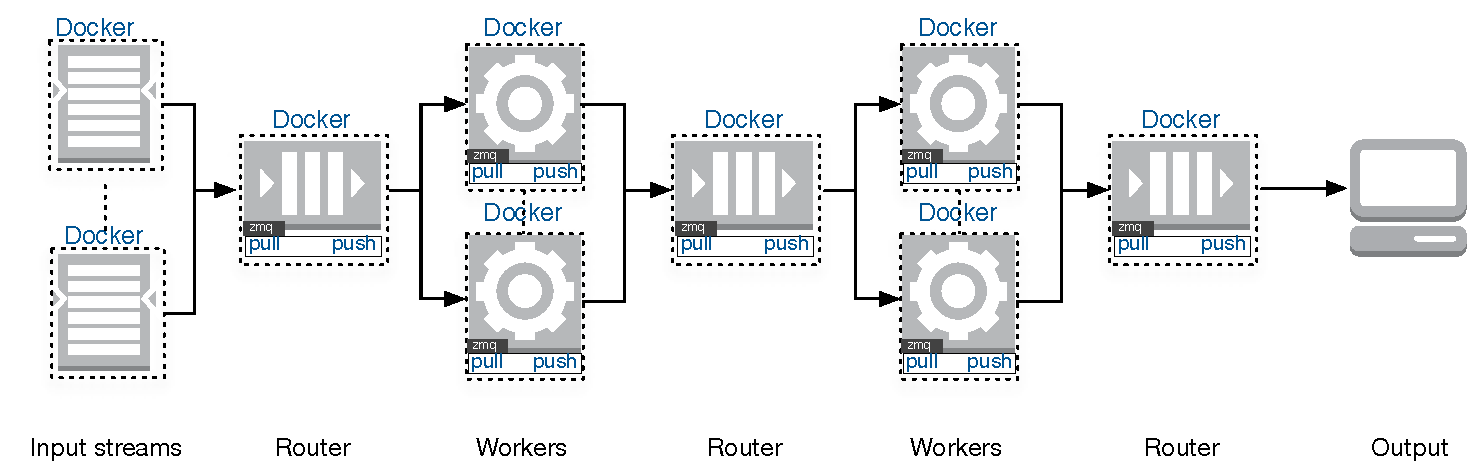
\includegraphics[width=.99\textwidth]{images/architecture_pipeline}
  \caption{Pipeline architecture.}
  \label{fig:architecture_pipeline}
\end{figure*}
